\documentclass[e3_tp3_main.tex]{subfiles}

\begin{document}

\chapter*{Introduction}

\label{chapter:intro}
\addcontentsline{toc}{chapter}{\nameref{chapter:intro}}

The FSM's implemented have the following characteristics:
\begin{itemize}
	\item Inputs: Signals whose value is independent from the FSM. There may be one or more.
	\item Outputs: Signals whose value depends on state variables only for Moore-type FSM's, and on both state variables and inputs for Mealy-type FSM's.
	\item State variables: Q value of flip-flops D which store the current state. There are as many as needed to represent the total number of states in binary format. These are written $y_0$, $y-1$, and so on.
	\item Next-state variables: Signals whose value represents the state that will be occurring in the next clock cycle. These are written as state variable but in capital letters: $Y_0$, $Y_1$, and so on. For example, if $Y_0=1$, in the next clock cycle $y_0=1$ independently of its current value. To achieve this, they are connected to the D input of the flip-flops.
\end{itemize}

All exercises were done according to the following pattern:
\begin{enumerate}
	\item Created the state diagram for both Moore and Mealy-type FSM's and checked that the second had fewer states than the first.
	\item Assigned state-variable values for each state.
	\item Created the state-transition table.
	\item Derived the Karnaugh maps for next-state variables and outputs from the state-transition table. In the case of Moore-type FSM's, the map for outputs depends only on the current state and not on the input, so it has fewer variables than the map for the next-state variables which depend on both. For Mealy-type FSM's, the next-state variables and the outputs depend on the same variables, therefore their maps are the same size.
	\item Obtained a sum-of-products expression from the map.
	\item Implemented the logic expression with AND and OR gates similarly to what would be obtained if a PLD was used (see figure \ref{fig:PLA}).
	\item Simulated the combinational logic in Verilog.
\end{enumerate}


\begin{figure}[h]
	\centering 
	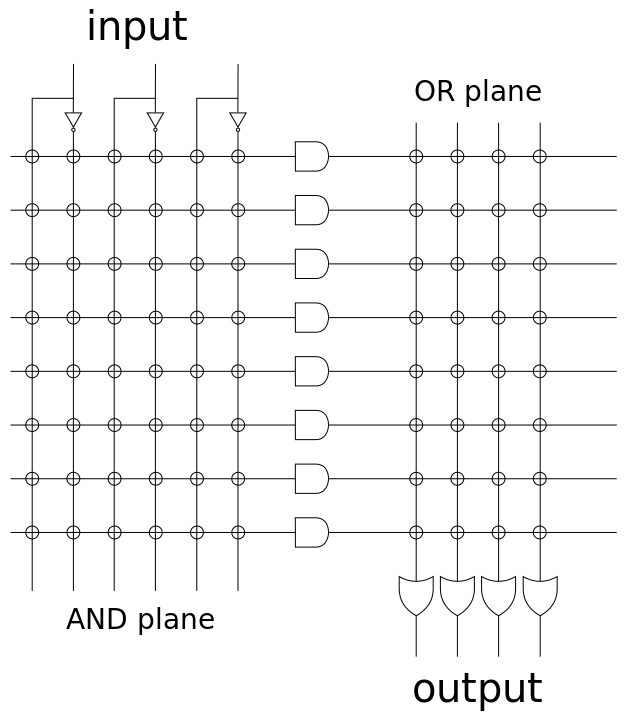
\includegraphics[scale=0.5]{PLD.png}
	\caption{PLA schematic for sum-of-products.}
	\label{fig:PLA}
\end{figure}



\end{document}